\documentclass[conference,a4paper]{IEEEtran}
\IEEEoverridecommandlockouts

\usepackage{cite}
\usepackage{amsmath,amssymb,amsfonts}
\usepackage{graphicx}
\usepackage{textcomp}
\usepackage{xcolor}
\usepackage{booktabs}
\usepackage{array}
\usepackage{multirow}
\usepackage{url}
\usepackage{tikz}
\usetikzlibrary{arrows.meta,positioning,fit,calc}
\usepackage{pgfplots}
\pgfplotsset{compat=1.18}
\usepackage[hidelinks]{hyperref}
% Page geometry matched to the IEEE A4 conference Word template:
% top 0.75in, bottom 1in, left/right 0.63in, column gap 0.25in
\usepackage[a4paper, top=54pt, bottom=72pt, left=45pt, right=45pt, columnsep=18pt]{geometry}
\def\IEEEkeywordsname{Keywords}


\def\BibTeX{{\rm B\kern-.05em{\sc i\kern-.025em b}\kern-.08em
    T\kern-.1667em\lower.7ex\hbox{\sc e}\kern-.125emX}}

\begin{document}

\title{IncidentMind: Cross-Topology Root Cause Analysis for Microservices with GraphSAGE, Learned Dispatch and LLM Agents}

\author{\setlength{\tabcolsep}{0pt}%
\begin{tabular*}{\textwidth}{@{\extracolsep{\fill}}ccc}
\begin{tabular}[t]{@{}c@{}}{\fontsize{11}{13}\selectfont Rakshitha Yathiraj}\\\textit{Dept. of Computer Science \& Engg.}\\\textit{B.M.S. College of Engineering}\\Bengaluru, India\\ rakshitha.raj004@gmail.com\end{tabular} &
\begin{tabular}[t]{@{}c@{}}{\fontsize{11}{13}\selectfont \textcolor{red}{Author Name}}\\\textit{Dept. of Computer Science \& Engg.}\\\textit{B.M.S. College of Engineering}\\Bengaluru, India\\ \textcolor{red}{email address}\end{tabular} &
\begin{tabular}[t]{@{}c@{}}{\fontsize{11}{13}\selectfont \textcolor{red}{Author Name}}\\\textit{Dept. of Computer Science \& Engg.}\\\textit{B.M.S. College of Engineering}\\Bengaluru, India\\ \textcolor{red}{email address}\end{tabular}
\end{tabular*}\\[12pt]
\begin{tabular*}{0.72\textwidth}{@{\extracolsep{\fill}}cc}
\begin{tabular}[t]{@{}c@{}}{\fontsize{11}{13}\selectfont \textcolor{red}{Author Name}}\\\textit{Dept. of Computer Science \& Engg.}\\\textit{B.M.S. College of Engineering}\\Bengaluru, India\\ \textcolor{red}{email address}\end{tabular} &
\begin{tabular}[t]{@{}c@{}}{\fontsize{11}{13}\selectfont \textcolor{red}{Author Name}}\\\textit{Dept. of Computer Science \& Engg.}\\\textit{B.M.S. College of Engineering}\\Bengaluru, India\\ \textcolor{red}{email address}\end{tabular}
\end{tabular*}}

\maketitle

\begin{abstract}
A microservice failure rarely stays where it starts. It travels along call edges, and the engineer on call ends up sifting through metrics from dozens of services to work out where it began. Graph-based root cause analysis (RCA) models do this well on the system they were trained on, but few papers ask what happens on a system they have never seen, and most stop at a ranked list of suspects. This paper describes IncidentMind, a pipeline in three parts: an inductive GraphSAGE scorer that ranks services by how likely each is to be the root cause, a Proximal Policy Optimisation (PPO) policy that chooses which service to investigate next within a step budget, and three LLaMA~3.2~3B agents, run locally, that read logs, metrics and recent commits and write a structured report. We train the scorer and the policy on RCAEval RE1 (Online Boutique, 11 services) and then, with no retraining, run them on ShopMind, a 12-service e-commerce testbed we built for fault injection. On held-out RE1 incidents the scorer puts the root cause first 92\% of the time, against 12\% for a training-free peer z-score baseline. On ShopMind it falls to 51\%, still six times the random rate of 8\%: 0.91 on CPU stress and 0.80 on memory pressure, but 0.08 on pod crashes, which we trace to error rate being constant zero in the training data. The learned dispatcher solves 57\% of ShopMind incidents within five steps where greedy dispatch solves 51\% (exact McNemar $p=0.031$). Pointed at the right service, the agent layer names the root cause in 82 of 100 incidents and abstains in 14. We also report four live fault-injection runs, one of them with two simultaneous faults, and release the testbed and the code.
\end{abstract}

\begin{IEEEkeywords}
root cause analysis, microservices, graph neural networks, GraphSAGE, reinforcement learning, LLM agents, AIOps
\end{IEEEkeywords}

%=====================================================================
\section{Introduction}
%=====================================================================
Cloud-native systems are assembled from small services that talk to each other over the network. The arrangement helps teams ship quickly, and it makes failures much harder to read. An authentication service starved of CPU surfaces as timeouts at the gateway; a payment service that has slowed down leaves its caller looking guilty~\cite{zhou2021fault,soldani2022survey}. Before anyone can fix anything, someone has to line up metrics, logs, traces and the last few deployments across services and work out where the trouble began.

Work on automated RCA has shifted from statistical correlation and causal inference~\cite{pham2024howfar,li2022circa} towards models that use the dependency graph itself~\cite{yu2021microrank,lee2023eadro,zhao2024chase}, and lately towards LLM agents that carry out the investigation~\cite{roy2024llmagents,chen2024rcacopilot,pei2025flowofaction,xu2025openrca}. Two gaps matter in practice. Graph models are almost always trained and tested on the same application, which says little about the case a team actually faces when it points the tool at its own system; Gao et al.~\cite{gao2025diagmlp} go further and ask whether the graph earns its place at all. And a ranked list is not an investigation. Someone still has to open the logs of whatever sits at the top, judge whether the evidence fits, and write the finding down.

IncidentMind is our attempt at both halves. GraphSAGE~\cite{hamilton2017graphsage} learns how to aggregate a node's neighbourhood instead of learning a transform tied to one adjacency matrix, so a trained model can score a graph it has never seen. A PPO policy~\cite{schulman2017ppo} reads the ranked scores together with what has already been checked, which means a wrong first guess is not the end of the search. Three specialist agents then investigate whichever service it picks. We claim four contributions:
\begin{itemize}
    \item \textbf{A pipeline in three layers} --- graph scoring, learned dispatch, LLM investigation --- whose state and action spaces are fixed in size, so one set of trained weights runs on graphs of different sizes.
    \item \textbf{A cross-topology evaluation with no leakage}: the models and the feature normalisation are fitted on RCAEval RE1~\cite{pham2025rcaeval} alone, and ShopMind is touched only at test time.
    \item \textbf{ShopMind}: twelve containerised services, four injectable faults, a frozen 100-incident set with ground-truth labels, and a path that injects a fault and captures it live.
    \item \textbf{A per-fault account of where the approach fails}, including pod crashes, which we diagnose rather than patch, together with three extensions aimed at deployment: multi-fault flagging, priority re-ranking and multi-instance telemetry.
\end{itemize}

%=====================================================================
\section{Related Work}
%=====================================================================
\textbf{Statistical and causal RCA.} Drain~\cite{he2017drain} and DeepLog~\cite{du2017deeplog} pick out unusual log events but know nothing about which service produced them. Causal methods such as CIRCA~\cite{li2022circa} rank candidates from dependencies between metrics. A benchmark study at ASE~2024~\cite{pham2024howfar} compared many of these and found none that holds up across systems and fault types; the benchmark that came out of that work, RCAEval~\cite{pham2025rcaeval}, supplies our training data.

\textbf{Graph-based fault localisation.} MicroRank~\cite{yu2021microrank} scores traces with spectrum analysis, Eadro~\cite{lee2023eadro} learns from logs, metrics and traces jointly, and CHASE~\cite{zhao2024chase} builds a causal heterogeneous graph. Nearly all of them are trained and evaluated on one application. Gao et al.~\cite{gao2025diagmlp} report that a plain MLP matches GNNs on current multimodal benchmarks, which is reason enough to ask what graph structure buys once the topology changes --- the experiment we run here.

\textbf{LLM agents for incidents.} RCACopilot~\cite{chen2024rcacopilot} and the study by Roy et al.~\cite{roy2024llmagents} show that LLMs can gather diagnostic evidence and propose causes in production. Flow-of-Action~\cite{pei2025flowofaction} steers a multi-agent system with standard operating procedures, while OpenRCA~\cite{xu2025openrca} finds that current models still struggle when handed raw telemetry. We narrow the search with a graph model before any prompt is sent, and keep the model local, so telemetry never leaves the organisation.

\textbf{Reinforcement learning in AIOps.} Most RL work in operations targets autoscaling and resource allocation; surveys of incident management~\cite{remil2024aiops} find little on learning the order in which to investigate. Our dispatcher is a small step in that direction.

%=====================================================================
\section{Problem Formulation}
%=====================================================================
A microservice system at time $t$ is a directed graph $G=(V,E)$ in which $V$ is the set of services and $(u,v)\in E$ means that $u$ calls $v$. Every service $v$ carries a feature vector $\mathbf{x}_v\in\mathbb{R}^5$: CPU usage, memory usage, mean latency, error rate and 99th-percentile latency. An incident $I=(G,\{\mathbf{x}_v\},r^*)$ has a single ground-truth root-cause service $r^*\in V$.

\textbf{Localisation.} A scorer $f$ returns $p_v=f(G,\mathbf{X})_v$, the probability that $v=r^*$, and orders $V$ by $p_v$ to give a ranking $\pi$. We report PR@$k=\mathbf{1}[r^*\in\pi_{1:k}]$ averaged over incidents, that is the top-$k$ hit rate, and MTTD, the mean rank of $r^*$ in $\pi$ --- how many services an engineer working down the list would open.

\textbf{Dispatch.} We treat investigation as an episodic decision process. At step $t$ the state $s_t$ holds the ranked scores and the services visited so far, and the action $a_t=(\text{agent},\text{slot})$ names an agent type and a rank slot. The episode ends when the chosen target is $r^*$, which counts as solved, or when the budget of $B=5$ steps runs out. The policy $\pi_\theta(a_t\mid s_t)$ should solve as many incidents as it can in as few steps as possible.

%=====================================================================
\section{IncidentMind Architecture}
%=====================================================================
Fig.~\ref{fig:arch} sketches the pipeline: telemetry arrives as a snapshot, GraphSAGE scores it, the PPO dispatcher picks a target, agents investigate it, and a report agent writes the result up.

\begin{figure}[t]
\centering
\resizebox{\columnwidth}{!}{%
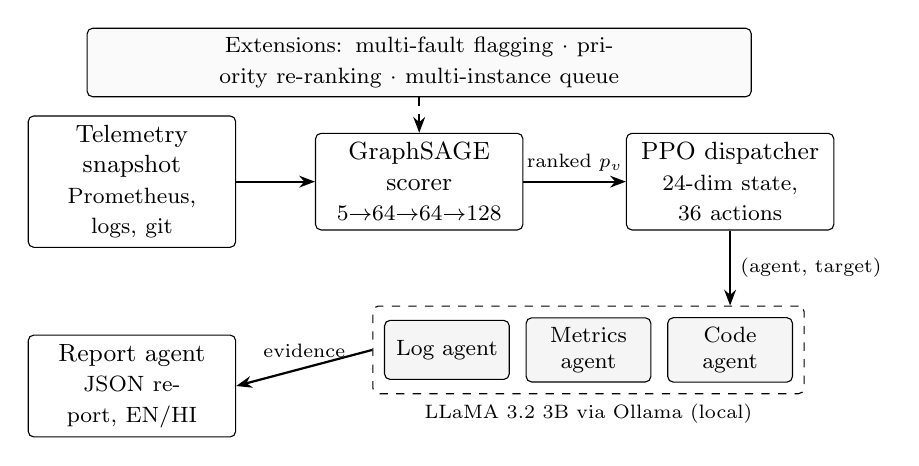
\begin{tikzpicture}[
  box/.style={draw, rounded corners=2pt, align=center, font=\small, minimum height=1.0cm, text width=2.4cm, fill=white},
  ag/.style={draw, rounded corners=2pt, align=center, font=\footnotesize, minimum height=0.75cm, text width=1.35cm, fill=gray!8},
  arr/.style={-{Stealth[length=2mm]}, thick}]
\node[box] (tel) {Telemetry snapshot\\ \footnotesize Prometheus, logs, git};
\node[box, right=1.0cm of tel] (gnn) {GraphSAGE scorer\\ \footnotesize 5$\to$64$\to$64$\to$128};
\node[box, right=1.3cm of gnn] (ppo) {PPO dispatcher\\ \footnotesize 24-dim state, 36 actions};
\node[box, above=0.45cm of gnn, text width=8.2cm, fill=gray!4, minimum height=0.6cm] (ext) {\footnotesize Extensions: multi-fault flagging $\cdot$ priority re-ranking $\cdot$ multi-instance queue};
\node[ag, below=1.1cm of ppo] (code) {Code agent};
\node[ag, left=0.2cm of code] (met) {Metrics agent};
\node[ag, left=0.2cm of met] (log) {Log agent};
\node[draw, dashed, rounded corners=2pt, fit=(log)(met)(code), inner sep=4pt] (agents) {};
\node[font=\scriptsize, below=0pt of agents] {LLaMA 3.2 3B via Ollama (local)};
\node[box, below=1.1cm of tel] (rep) {Report agent\\ \footnotesize JSON report, EN/HI};
\draw[arr] (tel) -- (gnn);
\draw[arr] (gnn) -- node[above, font=\scriptsize]{ranked $p_v$} (ppo);
\draw[arr] (ppo.south) -- node[right, font=\scriptsize]{(agent, target)} (ppo.south |- agents.north);
\draw[arr] (agents.west) -- node[above, font=\scriptsize]{evidence} (rep.east);
\draw[arr, dashed] (ext.south) -- (gnn.north);
\end{tikzpicture}}
\caption{IncidentMind pipeline. Only the scorer and dispatcher are learned; both are trained on RCAEval RE1 and applied unchanged to ShopMind.}
\label{fig:arch}
\end{figure}

\subsection{GraphSAGE Root-Cause Scorer}
The scorer is a three-layer GraphSAGE network~\cite{hamilton2017graphsage} with mean aggregation (widths $5\to64\to64\to128$, ReLU, dropout 0.2) and a linear two-class head on top. Every edge is added in both directions, because at inference time we do not know which way the fault is travelling and evidence has to be able to move from a cause down to its callers and back up again. Features are z-normalised with means and standard deviations fitted once on the training split and saved alongside the weights; they are never refitted on a test incident or on ShopMind. We learned that the hard way. With raw scales --- memory in bytes, error rate below one --- the logits saturated and training sat at a loss of $\ln 2$.

Training is node classification with class-weighted cross-entropy, the root-cause class carrying weight $|V|-1$ because each graph has exactly one positive node. We use Adam at learning rate 0.01 for 50 epochs, and take $p_v$ as the softmax probability of the root-cause class. Since a SAGE layer only ever looks at a node's own features and the mean of its neighbours', the same weights apply whatever the size or wiring of the graph.

\subsection{Learned Dispatch with PPO}
The observation is a fixed 24-dimensional vector: scores for the top 12 rank slots, zero-padded, followed by a 12-bit visited mask in the same slot order. There are $3\times12=36$ actions, one for each agent type and rank slot, with slots past the end of the graph wrapping modulo $|V|$. Acting on \emph{rank slots} instead of service names is the detail that lets a single policy run on the 11-node RE1 graph and on the 12-node ShopMind graph.

The reward is $+1$ when the chosen service is $r^*$, $-0.1$ for every step, and a further $-0.5$ for returning to a service already visited; episodes end on success or after five steps. We train with Stable-Baselines3~\cite{raffin2021sb3} PPO (MLP policy and value networks $[64,64]$, rollout 2048, batch 64, 10 epochs, $\gamma=0.99$, GAE $\lambda=0.95$, clip 0.2, entropy coefficient 0.01, learning rate $3\times10^{-4}$, 20{,}480 timesteps, seed 42) on the RE1 training split only, with the trained GraphSAGE scores as state.

\subsection{Investigation Agents}
Each agent is LLaMA~3.2~3B~\cite{grattafiori2024llama3}, served locally by Ollama at temperature 0, with a system prompt and a JSON schema to fill in. The \emph{log agent} reads recent container logs for the target service. The \emph{metrics agent} receives baseline and failure-window averages, and the deltas between them, for every service; the injected fault type never appears in a prompt. The \emph{code agent} summarises commits that touched the target. Each returns a finding, a severity, a confidence and the evidence behind it. Agents read from disk, so replayed and live data look identical to them.

\subsection{Report Agent}
The report agent folds the evidence bundle into one structured report: root-cause service, confidence, a summary of the evidence, a suggested fix, an estimated blast radius, and narrative text in English and Hindi. Where the evidence is thin it is allowed to answer \texttt{unknown}.

\subsection{Operational Extensions}
Three small additions aim at deployment rather than accuracy. \emph{Multi-fault flagging} lists every service scoring above 0.5 instead of surfacing the dispatch target alone. \emph{Priority re-ranking} multiplies the score by a static criticality weight ($w=1.0$ for auth, order, payment and the primary database, $0.6$ for the middle tier, $0.3$ for search, notification and the frontend) and reorders on the product, leaving the raw scores in the PPO state untouched. \emph{Multi-instance telemetry} adds a small HTTP receiver that stores snapshots tagged with the instance they came from, and a global queue that keys nodes on (instance, service) so two deployments of the same service are never confused.

%=====================================================================
\section{Experimental Setup}
%=====================================================================
\subsection{Datasets}
\textbf{RCAEval RE1-OB (training domain).} RE1~\cite{pham2025rcaeval} holds 125 Online Boutique~\cite{googleob} incidents: five root-cause services (ad, cart, checkout, currency, product catalogue) crossed with five faults (CPU, memory, disk, delay, packet loss), five repetitions each. We turn every incident into an 11-node, 15-edge graph using the published Online Boutique call graph, averaging features over the post-injection window, and split it 60/20/20 with seed 42 into 75 training, 25 validation and 25 test incidents. RE1 ships no error-rate metric, so that feature stays at zero throughout training --- a detail that matters later.

\textbf{ShopMind (unseen topology).} ShopMind is a 12-service e-commerce application we built for this study: an Nginx gateway, a web frontend, seven Node.js services (auth, user, order, payment, inventory, notification, search), a PostgreSQL primary and replica, and Redis, joined by 16 call edges. Services export Prometheus metrics and OpenTelemetry traces to Jaeger. Every application service exposes an \texttt{/inject-fault} endpoint with four faults behind it: \emph{CPU stress} (a busy loop for 80\,ms out of every 100\,ms), \emph{memory pressure} (bounded heap growth), \emph{network delay} (a 2\,s pause before handling a request) and \emph{pod crash} (\texttt{process.exit(1)}, re-triggered on restart until the fault window closes). Between incidents a settle check drives light load and waits for CPU below 0.15, mean latency below 100\,ms and error rate below 0.10, so that one incident does not bleed into the next. The frozen evaluation set has 100 incidents spread over all 28 service--fault pairs (23 CPU, 25 memory, 27 delay, 25 crash). Each incident is exported at the peak-anomaly snapshot of its failure window, with units converted to RE1 conventions (CPU in percent, latency in seconds, memory in bytes).

\subsection{Baselines}
For localisation we compare against a \emph{random} ranking and a training-free \emph{peer z-score} scorer, which ranks services by the root-mean-square z-score of their features against the other services in the same snapshot. For dispatch, every method sees the same GraphSAGE scores and the same five-step budget:
\begin{itemize}
    \item \textbf{Baseline A (random):} a uniform choice among unvisited services flagged anomalous ($p_v\ge0.5$).
    \item \textbf{Baseline B (threshold):} the first unvisited anomalous service in a per-incident shuffled arrival order, so that neither score order nor node position leaks the answer.
    \item \textbf{Baseline C (greedy):} the top-ranked service and nothing else; with no memory, a wrong first pick is never corrected.
\end{itemize}

\subsection{Metrics and Statistics}
We report PR@1/3/5 and MTTD for localisation, and solve rate and mean steps for dispatch, counting unsolved episodes at the budget. Confidence intervals for PR@$k$ are 95\% bootstrap intervals over 10{,}000 resamples, and dispatchers are compared with an exact McNemar test on paired per-incident outcomes. For the agent layer we report root-cause accuracy, how often it abstains with \texttt{unknown}, and JSON validity.

\subsection{Implementation}
The pipeline runs on Python~3.11 with PyTorch, PyTorch Geometric~\cite{fey2019pyg} and Stable-Baselines3; ShopMind runs under Docker Compose on a single laptop. Every learned number below comes from one pair of released checkpoints, and the unit-test suite covers the data contracts, the dispatch baselines and the cross-instance queue.

%=====================================================================
\section{Results}
%=====================================================================
\subsection{In-Domain Localisation (RE1 Test Split)}
Table~\ref{tab:loc} (left columns) shows GraphSAGE ranking the true root cause first in 23 of the 25 held-out RE1 incidents (PR@1 $=0.92$, 95\% CI $[0.80,1.00]$) and inside the top three in all of them (MTTD $=1.08$). The peer z-score scorer usually gets the root cause into the top three (0.72) but rarely to the top (0.12): on 21 of the 25 incidents it puts \emph{frontend} first, simply because the entry service is busy and its load deviates further from its peers than the faulty service does. Broken down by fault, GraphSAGE reaches PR@1 $=1.00$ on CPU, memory, disk and loss, and $0.33$ on delay, where the three incidents in the split still land inside the top three.

\begin{table}[t]
\centering
\caption{Root-cause localisation. RE1: 25 held-out test incidents (11 nodes). ShopMind: all 100 incidents (12 nodes), zero-shot with RE1-fitted models and normalisation.}
\label{tab:loc}
\setlength{\tabcolsep}{1.6pt}
\footnotesize
\begin{tabular}{lcccc@{\hspace{4pt}}cccc}
\toprule
 & \multicolumn{4}{c}{\textbf{RE1 (in-domain)}} & \multicolumn{4}{c}{\textbf{ShopMind (unseen)}} \\
\cmidrule(lr){2-5}\cmidrule(lr){6-9}
Method & PR@1 & PR@3 & PR@5 & MTTD & PR@1 & PR@3 & PR@5 & MTTD \\
\midrule
Random         & 0.09 & 0.27 & 0.45 & 6.00 & 0.08 & 0.25 & 0.42 & 6.50 \\
Peer z-score   & 0.12 & 0.72 & 0.80 & 3.28 & 0.18 & \textbf{0.77} & \textbf{0.78} & 3.84 \\
GraphSAGE      & \textbf{0.92} & \textbf{1.00} & \textbf{1.00} & \textbf{1.08} & \textbf{0.51} & 0.62 & 0.70 & \textbf{3.54} \\
\bottomrule
\end{tabular}
\end{table}

\subsection{Cross-Topology Transfer (ShopMind)}
Moved to ShopMind without retraining --- a system that differs from RE1 in service count, wiring, implementation language and fault mechanism --- GraphSAGE reaches PR@1 $=0.51$ ($[0.41,0.61]$), six times the random rate and nearly three times the z-score scorer at 0.18. The average hides most of the story, and Fig.~\ref{fig:perfault} breaks it apart. Transfer holds up for faults that push a resource metric on the faulty service itself, CPU stress at 0.91 and memory pressure at 0.80. It collapses for network delay (0.30) and pod crash (0.08).

The two failures fail differently. \emph{Network delay} makes the \emph{caller} look worse than the culprit: delay \emph{payment} in ShopMind and \emph{order} piles up pending requests, showing latency above 1.2\,s and timeout errors, while the delayed service itself can report span durations close to zero because clients give up before it answers. A scorer that follows symptoms gets pulled one hop upstream. \emph{Pod crash} leaves the crashed service with zeroed resource and latency metrics and an error rate of 1.0, while its caller --- usually \emph{order} --- carries the raised latency and errors. Since error rate is constant zero across RE1, the model never learned to read that signal, and a node of zeros looks \emph{less} anomalous than its busy neighbours; on the remaining four features it is also indistinguishable from uninstrumented nodes such as the gateway. The untrained z-score scorer, by contrast, puts the crashed service in the top three on 96\% of crash incidents, because an error rate of 1.0 sitting next to zeroed metrics stands out from its peers with no training at all. The two signals look complementary. We prefer to report this as a limitation of the training data rather than bolt on a hand-written crash rule, which would hollow out the transfer claim.

\begin{figure}[t]
\centering
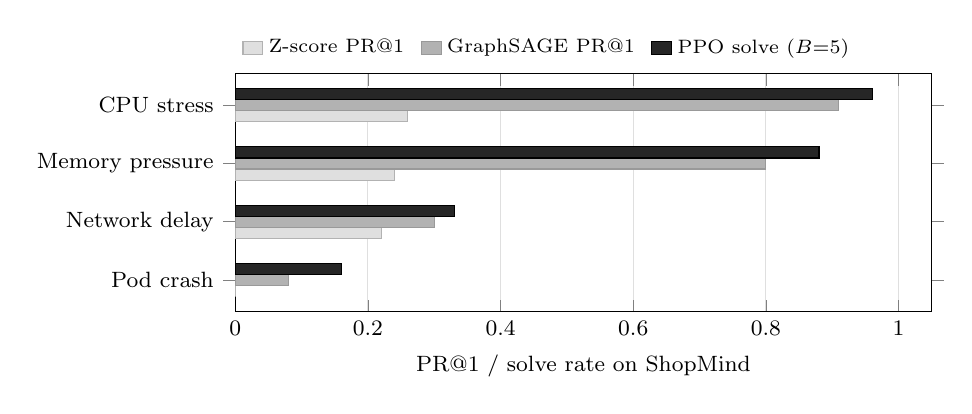
\begin{tikzpicture}
\begin{axis}[
    xbar=0pt, bar width=4pt, width=0.86\columnwidth, height=4.6cm,
    xmin=0, xmax=1.05, xlabel={PR@1 / solve rate on ShopMind},
    symbolic y coords={Pod crash, Network delay, Memory pressure, CPU stress},
    ytick=data, y tick label style={font=\footnotesize},
    x tick label style={font=\footnotesize}, xlabel style={font=\footnotesize},
    legend style={font=\scriptsize, legend columns=3, at={(0.45,1.02)}, anchor=south, draw=none, /tikz/every even column/.append style={column sep=4pt}},
    legend image code/.code={\draw[#1] (0cm,-0.08cm) rectangle (0.25cm,0.08cm);},
    reverse legend=false,
    enlarge y limits=0.18, xmajorgrids, grid style={gray!25}]
\addplot[fill=gray!25, draw=gray!60] coordinates {(0.00,Pod crash) (0.22,Network delay) (0.24,Memory pressure) (0.26,CPU stress)};
\addplot[fill=gray!60, draw=gray!80] coordinates {(0.08,Pod crash) (0.30,Network delay) (0.80,Memory pressure) (0.91,CPU stress)};
\addplot[fill=black!85, draw=black] coordinates {(0.16,Pod crash) (0.33,Network delay) (0.88,Memory pressure) (0.96,CPU stress)};
\legend{Z-score PR@1, GraphSAGE PR@1, PPO solve ($B{=}5$)}
\end{axis}
\end{tikzpicture}
\caption{Per-fault zero-shot results on ShopMind ($n=23/25/27/25$ for CPU/memory/delay/crash).}
\label{fig:perfault}
\end{figure}

\subsection{Learned Dispatch}
Table~\ref{tab:dispatch} compares dispatchers working from identical scores. On RE1 the scorer is accurate enough that almost everything is solved by everything; PPO uses the fewest steps among the methods that solve all 25 (1.08), while greedy dispatch loses the two incidents whose root cause sat at rank two.

ShopMind separates them further. PPO solves 57\% of incidents within five steps, against 51\% for greedy and 45\% for the random and threshold baselines, and mean steps drop from 2.96 to 2.78. Paired incident by incident, PPO solves six that greedy misses and misses none that greedy solves (exact McNemar $p=0.031$); the gain sits on the harder faults, at +0.08 on pod crash, +0.04 on network delay and +0.08 on memory pressure. Tracing episodes shows exactly what the policy learned. It opens at rank~1 and, if that misses, tries rank~2 --- all 57 solves land on step 1 or 2. It never explores past the second slot: in the other 43 episodes it cycles between ranks~1 and~2 until the budget expires, revisit penalty notwithstanding. The gain, then, is a learned second guess, and nothing it does can recover a root cause ranked third or lower. Deeper search would need a richer state, score gaps or per-feature evidence returned by the agents. Baselines A and B are held back by a different problem: only 0.78 services per incident cross the 0.5 threshold on ShopMind, so they run out of candidates.

\begin{table}[t]
\centering
\caption{Dispatch under a five-step budget with identical GraphSAGE scores. Steps: mean over all incidents, unsolved counted as 5.}
\label{tab:dispatch}
\setlength{\tabcolsep}{4pt}
\begin{tabular}{lcccc}
\toprule
 & \multicolumn{2}{c}{\textbf{RE1 test ($n=25$)}} & \multicolumn{2}{c}{\textbf{ShopMind ($n=100$)}} \\
\cmidrule(lr){2-3}\cmidrule(lr){4-5}
Dispatcher & Solve & Steps & Solve & Steps \\
\midrule
A: random (anomalous)   & 1.00 & 1.12 & 0.45 & 3.27 \\
B: threshold, arrival   & 1.00 & 1.12 & 0.45 & 3.24 \\
C: greedy top-1         & 0.92 & 1.32 & 0.51 & 2.96 \\
PPO (ours)              & \textbf{1.00} & \textbf{1.08} & \textbf{0.57} & \textbf{2.78} \\
\bottomrule
\end{tabular}
\end{table}

\subsection{Agent Layer}
To look at the LLM layer on its own, free of localisation errors, we dispatched the metrics and report agents straight to the ground-truth service on a separate run of 100 ShopMind incidents with raw telemetry series, withholding the fault type from the prompts. Table~\ref{tab:agents} has the outcome: the report named the correct root cause in 82 incidents, answered \texttt{unknown} in 14 and named the wrong service in 4, and all 100 reports parsed as valid JSON. Memory pressure was perfect at 28/28, pod crash weakest at 16/23, and all four wrong answers were a fault on \emph{notification-service} attributed to \emph{auth-service}. Stated confidence turned out to be informative: it averaged 0.69 where the answer was right and 0.11 where it was wrong or withheld. Because this run is handed the correct target, it is an upper bound --- end to end, the agents inherit whatever the scorer and dispatcher get wrong.

\begin{table}[t]
\centering
\caption{Agent-layer accuracy under oracle dispatch (100 ShopMind incidents).}
\label{tab:agents}
\begin{tabular}{lcccc}
\toprule
Fault & $n$ & Correct & Unknown & Wrong \\
\midrule
CPU stress       & 32 & 25 (78\%)  & 7 & 0 \\
Memory pressure  & 28 & 28 (100\%) & 0 & 0 \\
Network delay    & 17 & 13 (76\%)  & 3 & 1 \\
Pod crash        & 23 & 16 (70\%)  & 4 & 3 \\
\midrule
\textbf{All}     & 100 & \textbf{82 (82\%)} & 14 & 4 \\
\bottomrule
\end{tabular}
\end{table}

\subsection{Live End-to-End Runs}
We also ran the whole pipeline against live faults: inject, capture five baseline and 15 failure snapshots two seconds apart, pick the peak snapshot, score, dispatch, investigate, report. Table~\ref{tab:live} lists the four runs from the final integrated build. GraphSAGE ranked the injected service first in each of them, PPO dispatched to it on the opening step, and the report named it with confidence 0.8. The dual-fault run put CPU stress on \emph{order} and \emph{inventory} at once; both scored 1.00 and multi-fault flagging listed both, where the dispatch target on its own would have surfaced only one.

\begin{table}[t]
\centering
\caption{Live end-to-end runs on ShopMind (final build).}
\label{tab:live}
\setlength{\tabcolsep}{3pt}
\begin{tabular}{llccc}
\toprule
Fault & Injected service(s) & Rank-1 score & PPO step & Report \\
\midrule
CPU stress     & auth              & 1.00 & 1 & correct \\
CPU stress     & order             & 1.00 & 1 & correct \\
Network delay  & payment           & 1.00 & 1 & correct \\
Dual CPU       & order + inventory & 1.00 / 1.00 & 1 & correct$^\dagger$ \\
\bottomrule
\multicolumn{5}{l}{\footnotesize $^\dagger$Report names \emph{order}; multi-fault flag lists both services.}
\end{tabular}
\end{table}

Two earlier runs show the extensions at work and the main weakness in the open. In a CPU-stress run on \emph{auth}, GraphSAGE scored \emph{auth} and \emph{notification} at 1.00 apiece; priority re-ranking held \emph{auth} (high tier) at the top and pushed \emph{notification} (low tier) down. In a live pod-crash run on \emph{auth}, the scorer put \emph{payment} first on nothing more than a small CPU fluctuation (score 0.45), and the dispatcher, the agents and the report all followed it there with confidence 0.5 --- the offline pod-crash result reproduced live. On the 100-incident benchmark, priority re-ranking moved PR@1 from 0.51 to 0.48 and left PR@5 at 0.70. That is the intended behaviour: it reorders by business impact, and it does not make the scorer more accurate.

%=====================================================================
\section{Discussion and Limitations}
%=====================================================================
\textbf{What transfers.} The gap between in-domain and cross-domain accuracy (PR@1 of 0.92 against 0.51) is wide, and some of the in-domain figure is likely easy marks: RE1 has one fixed topology and only five root-cause services, which a model can partly memorise. The per-fault view says more than the average. Faults whose signature lands on the faulty node itself transfer nearly intact; faults whose signature shows up on a neighbour, or in a feature that was flat during training, do not. Graph structure on its own does not solve cross-topology RCA. The most direct fix is to train on richer sources, RCAEval RE2/RE3 with logs and traces among them.

\textbf{Report quality.} Attribution held up whenever the evidence was clear, but the free-text portions were weaker. A few suggested fixes recycled harmless log lines --- a service ``listening on a port'' --- as causes, one CPU-stress report mentioned pod crashes that never happened, and the Hindi text sometimes repeated itself. None of this is surprising from a 3B model. The structured fields deserve more trust than the narrative, and we did not evaluate translation quality formally.

\textbf{Threats to validity.} The RE1 test split holds only 25 incidents, which leaves its confidence intervals wide. ShopMind is a controlled testbed with four fault types and one instance per service. The agent evaluation used oracle dispatch on a separately generated incident set, so it is not an end-to-end accuracy figure. The live runs are case studies, not a benchmark. Multi-instance support was verified over loopback; a real cross-machine run, and the notification hooks, remain future work. Finally, RE1 features are window averages while ShopMind uses peak snapshots, which adds a further distribution shift on top of the topology change.

%=====================================================================
\section{Conclusion}
%=====================================================================
IncidentMind puts an inductive GraphSAGE scorer, a PPO dispatcher defined over rank slots and local LLM agents into one pipeline that runs unchanged on a topology it never saw in training. Trained on RCAEval RE1 alone, it localises root causes on ShopMind at six times the random rate, transfers well on resource faults, and fails on crashes for a reason we can name: the signal was missing from the training data. Learned dispatch recovers significantly more incidents than greedy dispatch by learning a second guess, and given the right target the agent layer produces a correct, machine-readable report 82\% of the time. The obvious next steps are training on multimodal sources to close the crash and delay gaps, combining the learned and statistical scores, which look complementary, and a genuine multi-machine deployment. Code and testbed are at \url{https://github.com/rakshithay3/incident-mind}.

\section*{Acknowledgment}
The authors thank the Department of Computer Science and Engineering, B.M.S. College of Engineering, Bengaluru, for the facilities and support provided for this work. We also thank the authors of RCAEval for releasing their benchmark data publicly, and the maintainers of PyTorch Geometric, Stable-Baselines3 and Ollama, whose open-source tools made this study possible.

The authors used Claude (Anthropic), an AI assistant, to write the analysis scripts that computed the metrics in Tables~\ref{tab:loc}--\ref{tab:dispatch} and Fig.~\ref{fig:perfault} from the authors' trained models and datasets. The IncidentMind system, the ShopMind testbed, model training, the agent evaluation and the live fault-injection runs are the authors' own work. The authors reviewed and checked all AI-generated content and take full responsibility for the paper.

\begin{thebibliography}{99}

\bibitem{zhou2021fault}
X.~Zhou, X.~Peng, T.~Xie, J.~Sun, C.~Ji, W.~Li, and D.~Ding, ``Fault analysis and debugging of microservice systems: Industrial survey, benchmark system, and empirical study,'' \emph{IEEE Trans. Softw. Eng.}, vol.~47, no.~2, pp.~243--260, 2021.

\bibitem{soldani2022survey}
J.~Soldani and A.~Brogi, ``Anomaly detection and failure root cause analysis in (micro)service-based cloud applications: A survey,'' \emph{ACM Comput. Surv.}, vol.~55, no.~3, 2022.

\bibitem{pham2024howfar}
L.~Pham, H.~Ha, and H.~Zhang, ``Root cause analysis for microservices based on causal inference: How far are we?'' in \emph{Proc. 39th IEEE/ACM Int. Conf. Automated Software Engineering (ASE)}, 2024.

\bibitem{li2022circa}
M.~Li, Z.~Li, K.~Yin, X.~Nie, W.~Zhang, K.~Sui, and D.~Pei, ``Causal inference-based root cause analysis for online service systems with intervention recognition,'' in \emph{Proc. 28th ACM SIGKDD Conf. Knowledge Discovery and Data Mining}, 2022.

\bibitem{yu2021microrank}
G.~Yu, P.~Chen, H.~Chen, Z.~Guan, Z.~Huang, L.~Jing, T.~Weng, X.~Sun, and X.~Li, ``MicroRank: End-to-end latency issue localization with extended spectrum analysis in microservice environments,'' in \emph{Proc. Web Conf. (WWW)}, 2021.

\bibitem{lee2023eadro}
C.~Lee, T.~Yang, Z.~Chen, Y.~Su, and M.~R.~Lyu, ``Eadro: An end-to-end troubleshooting framework for microservices on multi-source data,'' in \emph{Proc. 45th Int. Conf. Software Engineering (ICSE)}, 2023.

\bibitem{zhao2024chase}
Z.~Zhao, T.~Zhang, Z.~Shen, H.~Dong, X.~Ma, X.~Liu, and Y.~Yang, ``CHASE: A causal heterogeneous graph based framework for root cause analysis in multimodal microservice systems,'' arXiv:2406.19711, 2024.

\bibitem{roy2024llmagents}
D.~Roy, X.~Zhang, R.~Bhave, C.~Bansal, P.~Las-Casas, R.~Fonseca, and S.~Rajmohan, ``Exploring LLM-based agents for root cause analysis,'' in \emph{Companion Proc. 32nd ACM Int. Conf. Foundations of Software Engineering (FSE)}, 2024.

\bibitem{chen2024rcacopilot}
Y.~Chen, H.~Xie, M.~Ma, Y.~Kang, X.~Gao, L.~Shi, Y.~Cao, X.~Gao, H.~Fan, M.~Wen, J.~Zeng, S.~Ghosh, X.~Zhang, C.~Zhang, Q.~Lin, S.~Rajmohan, D.~Zhang, and T.~Xu, ``Automatic root cause analysis via large language models for cloud incidents,'' in \emph{Proc. 19th European Conf. Computer Systems (EuroSys)}, 2024.

\bibitem{pei2025flowofaction}
C.~Pei, Z.~Wang, F.~Liu, Z.~Li, Y.~Liu, X.~He, R.~Kang, T.~Zhang, J.~Chen, J.~Li, G.~Xie, and D.~Pei, ``Flow-of-Action: SOP enhanced LLM-based multi-agent system for root cause analysis,'' in \emph{Companion Proc. ACM Web Conf. (WWW)}, 2025.

\bibitem{xu2025openrca}
J.~Xu \emph{et al.}, ``OpenRCA: Can large language models locate the root cause of software failures?'' in \emph{Proc. Int. Conf. Learning Representations (ICLR)}, 2025.

\bibitem{gao2025diagmlp}
F.~Gao, R.~Xin, X.~Li, and Y.~Zhang, ``Are GNNs actually effective for multimodal fault diagnosis in microservice systems?'' arXiv:2501.02766, 2025.

\bibitem{hamilton2017graphsage}
W.~L.~Hamilton, R.~Ying, and J.~Leskovec, ``Inductive representation learning on large graphs,'' in \emph{Advances in Neural Information Processing Systems (NeurIPS)}, vol.~30, 2017.

\bibitem{schulman2017ppo}
J.~Schulman, F.~Wolski, P.~Dhariwal, A.~Radford, and O.~Kavukcuoglu, ``Proximal policy optimization algorithms,'' arXiv:1707.06347, 2017.

\bibitem{pham2025rcaeval}
L.~Pham, H.~Zhang, H.~Ha, F.~Salim, and X.~Zhang, ``RCAEval: A benchmark for root cause analysis of microservice systems with telemetry data,'' in \emph{Companion Proc. ACM Web Conf. (WWW)}, 2025.

\bibitem{he2017drain}
P.~He, J.~Zhu, Z.~Zheng, and M.~R.~Lyu, ``Drain: An online log parsing approach with fixed depth tree,'' in \emph{Proc. IEEE Int. Conf. Web Services (ICWS)}, 2017.

\bibitem{du2017deeplog}
M.~Du, F.~Li, G.~Zheng, and V.~Srikumar, ``DeepLog: Anomaly detection and diagnosis from system logs through deep learning,'' in \emph{Proc. ACM SIGSAC Conf. Computer and Communications Security (CCS)}, 2017.

\bibitem{remil2024aiops}
Y.~Remil, A.~Bendimerad, R.~Mathonat, and M.~Kaytoue, ``AIOps solutions for incident management: Technical guidelines and a comprehensive literature review,'' arXiv:2404.01363, 2024.

\bibitem{grattafiori2024llama3}
A.~Grattafiori \emph{et al.}, ``The Llama 3 herd of models,'' arXiv:2407.21783, 2024.

\bibitem{googleob}
Google Cloud Platform, ``Online Boutique: Cloud-native microservices demo application,'' GitHub repository. [Online]. Available: \url{https://github.com/GoogleCloudPlatform/microservices-demo}

\bibitem{raffin2021sb3}
A.~Raffin, A.~Hill, A.~Gernhardt, M.~Ernestus, and N.~Dormann, ``Stable-Baselines3: Reliable reinforcement learning implementations,'' \emph{J. Mach. Learn. Res.}, vol.~22, no.~268, pp.~1--8, 2021.

\bibitem{fey2019pyg}
M.~Fey and J.~E.~Lenssen, ``Fast graph representation learning with PyTorch Geometric,'' in \emph{ICLR Workshop on Representation Learning on Graphs and Manifolds}, 2019.

\end{thebibliography}

\end{document}
